Para el plan de pruebas se construyeron dos opciones para la transmisión de energía con las antenas que buscan explorar aspectos distintos del sistema. Por un lado, el CAERCEM del itba posee un transmisor en la banda UHF de hasta 20W que podríamos utilizar para aislar al sistema de recepción. Por otro lado, para probar el sistema de transmisión y recepción en conjunto, se utilizará un módulo oscilador HM-TRPW-RS232 en 915MHz en cascada con un amplificador de potencia apto para radiofrecuencia que será alimentado mediante una etapa DC-DC conectado a la batería de la unidad de energía. La salida del amplificador será llevada hasta la antena transmisora utilizando cable mallado RG-213 apto para radiofrecuencia y de bajas pérdidas.

\begin{figure}[H]
	\centering
	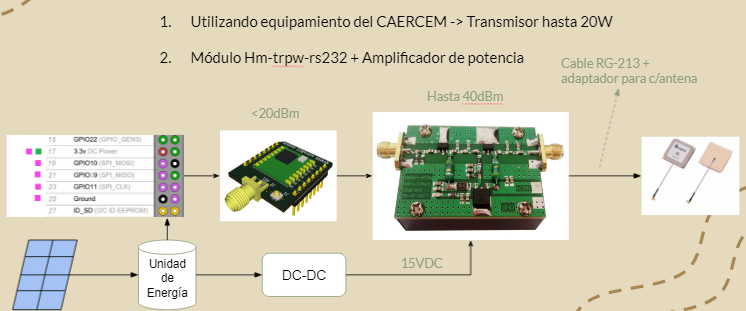
\includegraphics[width=0.9\linewidth]{ImagenesIngenieria de Detalle/planDePruebasAntenasA}	
	\caption{Plan de pruebas Antenas A.}
	\label{fig:planDePruebasAntenasA}
\end{figure}

Del lado de la recepción, se conectará la antena receptora a la placa de evaluación del P1110 y se medirá la tensión en el supercapacitor provisto en esta. Conociendo la capacitancia y el valor de tensión a lo largo del tiempo se puede validar la potencia recibida.


\begin{figure}[H]
	\centering
	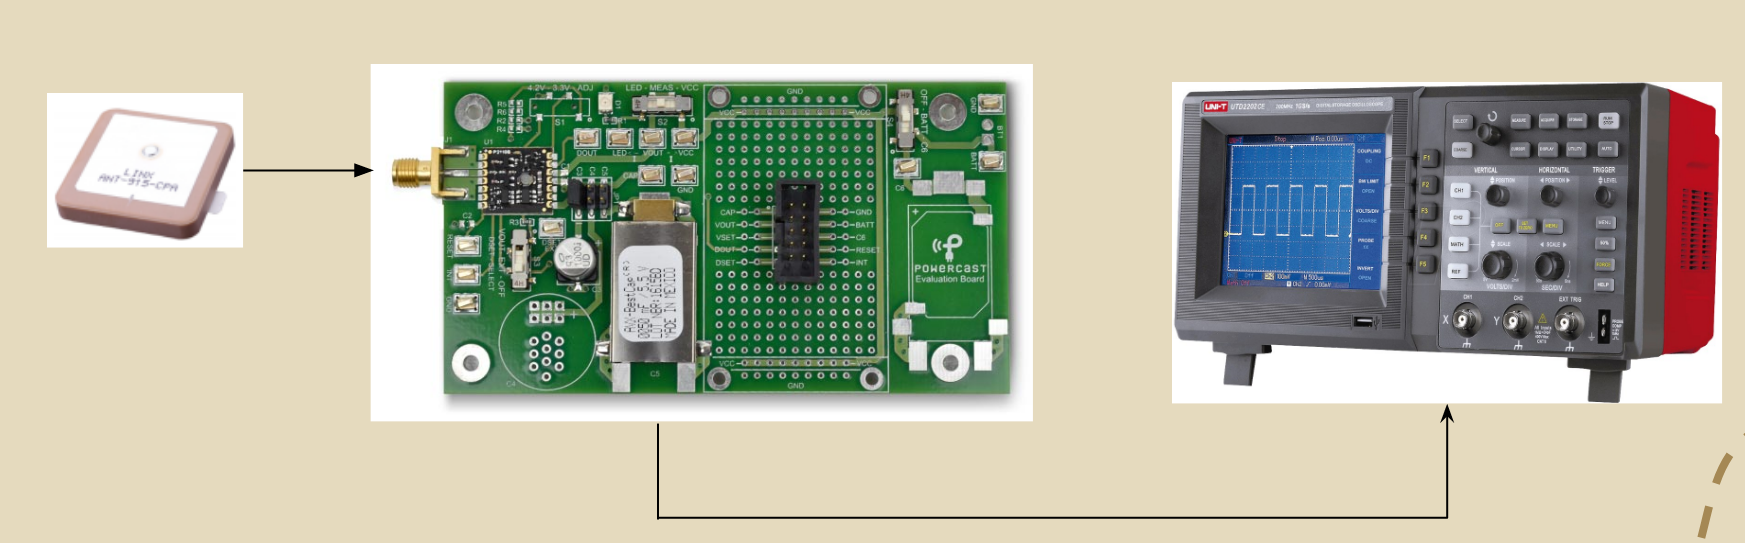
\includegraphics[width=0.8\linewidth]{ImagenesIngenieria de Detalle/planDePruebasAntenasB}	
	\caption{Plan de pruebas Antenas B.}
	\label{fig:planDePruebasAntenasB}
\end{figure}

En cuanto a los sensores se comparan los resultados de los sensores del sistema contra unos previamente calibrados.

\begin{figure}[H]
	\centering
	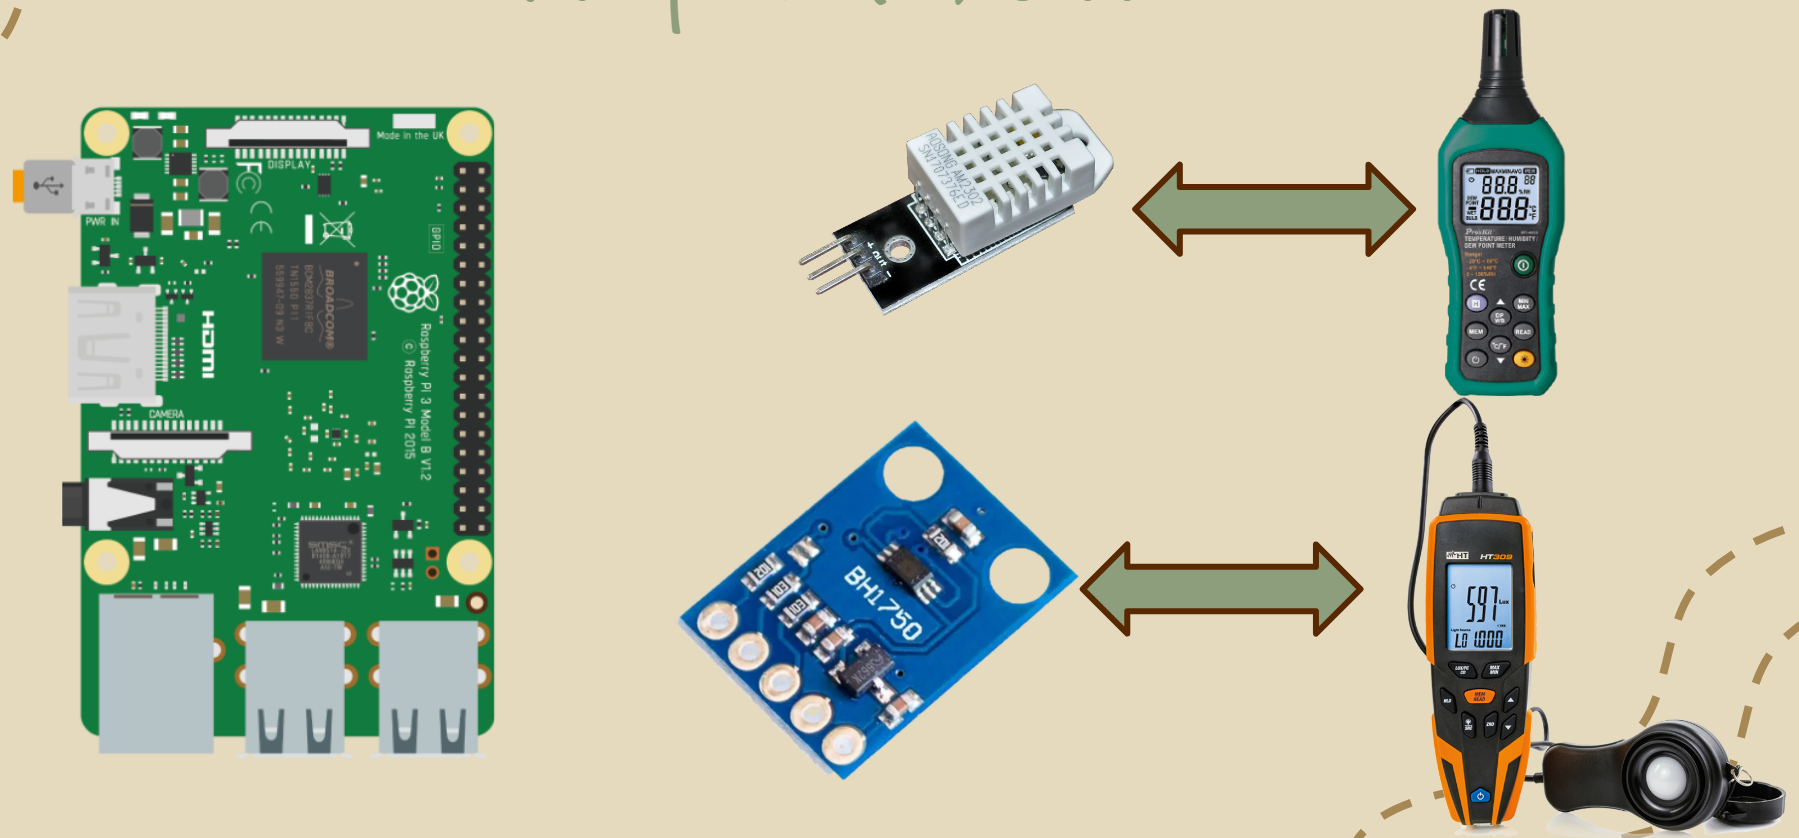
\includegraphics[width=0.8\linewidth]{ImagenesIngenieria de Detalle/planDePruebasSensores}	
	\caption{Plan de pruebas sensores.}
	\label{fig:planDePruebasSensores}
\end{figure}